\chapter{Data}
\label{chapter:data}

From section~\ref{sec:t-cell/activation} we gather that analysing the intracellular \Calcium concentration gives us good insight in wheter and when a cell activates. Additionally it can be measured relatively easily by the method described in this chapter.

\section{Structure of Data}

The data matrix has a row per tracked cell and frame. The information stored for each cell and frame combination is described in detail in table~\ref{tab:information_data_matrix}.

\begin{table}[h!]
	\centering
	\begin{tabular}{|c|c|l|}
		\hline
		\textbf{Name} & \textbf{Data Type} & \textbf{Description} \\
		\hline
		x & float64 & Position of cell in pixels along the horizontal axis \\
		\hline
		y & float64 & Position of cell in pixels along the vertical axis \\
		\hline
		frame & int32 & Number of frame, with frame rate of 1 frame per second \\
		\hline
		mass short & float64 & Brightness of cell in 340nm channel \\
		\hline
		bg short & float64 & Background in 340nm channel \\
		\hline
		mass long & float64 & Brightness of cell in 380nm channel \\
		\hline
		bg long & float64 & Background in 380nm channel \\
		\hline
		ratio & float64 & Calculated as mass short divided by mass long \\
		\hline
		particle & int32 & Identification for each particle \\
		\hline
	\end{tabular}
	\caption{Description and data type of all columns present in the data matrix.}
	\label{tab:information_data_matrix}
\end{table}

% mouse pos: 4289, 720; mouse neg: 7683, 785; human pos: 694, 948

One recording can have between 500 and 10000 cells and is between 700 and 1000 frames long, which corresponds to between about 11 and 17 minutes. The ratio is typically between 0 and 5.


\section{How it was generated}

exprimental setup, what types of t cells where used?, apc layer, explain steps in experiment

\subsection{Jurkat Cells, 5c.c7 primary mouse T cells and Fura-2}

The prototypical cell line to study T cell signaling is the Jurkat cell line.\cite{morgan2023} It was obtained from the blood of a boy with T cell leukemia.\cite{schneider1977} Different cell lines within the Jurkat family are described by Abraham and Weiss.\cite{abraham2004} They provide a timeline of discoveries linked to Jurkat cells and t cell receptor signalling.

describe which mouse t cells are used

In order to be able to measure the intracellular \Calcium concentration of cells they can be labelled with Fura-2. This method provides a way to record the \Calcium concentration of multiple cells over a time period.\cite{martinez2017} Challenges encountered when using Fura-2 on certain cell types are described by Roe, Lemasters and Herman along with their respective solutions.\cite{roe1990}

\subsection{Measuring Calcium Concentration}

After the cells have been labeled with Fura-2 an recording of up to 15 minute can be generated. To achieve this the cells and stimulant are photographed at both 340nm and 380nm wavelength once per second. The resolution of the images are 1.6um per pixel. By calculating the ratio of the two images at each point the \Calcium concentration can be observed. An examplary resulting image showing the ratio is shown in figure~\ref{fig:example_ratio_img}. The T cells are appear a lighter shade than the background.

\begin{figure}
	\centering
	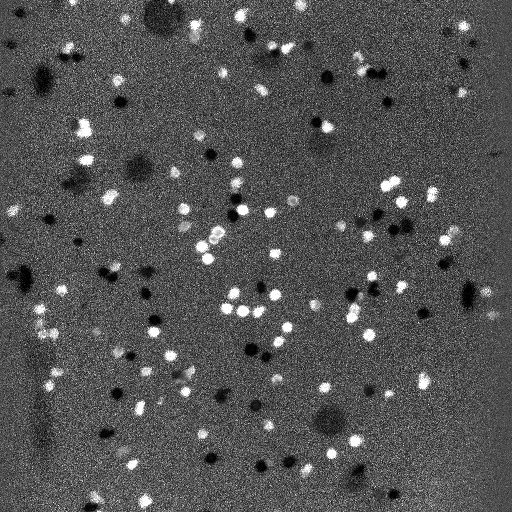
\includegraphics[width=0.6\linewidth]{fig/frame_ratio.jpg}
	\caption{Single frame showing the ratio of the 340nm and 380nm images from a recording of human Jurkat cells. Activated cells apear lighter, unactivated cells darker than the background. Big dark circles are out of focus cells that have not yet settled on to the plate.}
	\label{fig:example_ratio_img}
\end{figure}

To activate the cells in the duration of the recording they are transfered to a plate covered with replicas of the MHC-peptide complex normally present on APCs. For a negative control the plate is not covered with peptides, while for the positive control the plate is covered very densly. Recordings of different densities in peptides lead to activation of only some of the t cells.

\subsection{Processing}

To track single t cells moving around during the video the sum of the 340nm and 380nm image for each second is calculated. In this image it is easier to separate t cells from the background. Therefore it is used to track the movement of cells. Each cell is numbered, such that the same cell will have the same number during as much of the video as possible. The position and shade during both 340nm and 380nm as well as the ratio of each particle and each frame is then recorded into the data structure used in this work. The first 50 frames at the start of the recording are discarded due to the video being out of focus. Additionally cells only appearing in fewer than 20 frames are discarded as they most likely represent trackactories incorrectly tracked.
